\section{Pinch in the Reverse Field Pinch}\label{sec:eb_pinch}
%\section{Observations of inward pinch flow associated with $\vec{E}\times\vec{B}$ drift and it's effect on ion thermal transport}

%In previous power balance work, the heat lost to particle flow is one of the largest terms\cite{Fiksel2006}. Calculating $P_{flow}$ involves estimating the ion particle flux.  However, no diagnostic measurements of $n_i$ in MST is available, therefore, $n_i$ is inferred indirectly through the evolution of $n_e$ combined with previous work on characterizing the impurity content in PPCD\cite{Kumar2012,Nornberg2018IncorporatingCharge}.

%...

%Given that the  calculated electron source rates are insufficient to account for the density rise, another possibility is an inward particle flux. The particle flux ($\Gamma_{obs}$) needed to satisfy the continuity equation (\ref{eqn:cont}) is then calculated. However, we seek to confirm the theoretical plausibility of an inward pinch by considering the evolution of the magnetic equilibrium.

%There is currently no diagnostic that measures the poloidal and toroidal $\vec{E}$, which is needed to constrain the radial $\Gamma_{\vec{E}\times\vec{B}}$. Instead, the slow time-scale E field is estimated using the evolution of reconstructed B field from edge flux coil and FIR polarimetry data. The radial flux, $\Gamma_{\rho} = n_e\frac{(\Vec{E}\times\Vec{B})_{\rho}}{B^2}$, is constrained by $E_{pol}$ and $E_{tor}$. The MSTfit equilibrium reconstruction outputs reconstructed flux values and flux surfaces in 2D which enables the calculation of $E_{pol}$ and $E_{tor}$. In particular $E_{pol}$ can be calculated through:

%\begin{align}
%   E_{pol}(\rho_v) & = -\frac{1}{\rho_v}\int_{0}^{\rho_v}\rho_v' \frac{dB_{tor}}{dt} d\rho_v'
%\end{align}

%where it is taken as a boundary condition that the $E_{pol}$ is zero at the magnetic axis.

%where $\rho_v$ is the flux surface averaged minor radius.

%Calculating $E_{tor}$ is slightly more complicated, as it is a function of major radius and not $\rho$. On MST, there is a poloidal gap (a cut in the vessel in the poloidal plane) in the conducting wall and the voltage measured across the gap ($V_{PG}$) is a reflection of the inductively driven toriodal E field. To incorporate into the 1-D approximation, $E_{tor}(R, Z=0)$ along the Z = 0 plane is determined as a function of major radius (R) through:

%\begin{align}
%\oint_S \vec{E}\cdot d\vec{l} &= -\iint \frac{\partial}{\partial t}\vec{B}\cdot d\vec{s}\\
%E_{tor}(R) 2\pi R &= -\int_0^{2\pi}\int_{R_{in}}^{R}R'\frac{\partial B_{pol}}{\partial t} d\phi'dR' - V_{PG}\\
%E_{tor}(R) &= -\frac{1}{R}\int_{R_{in}}^{R}R'\frac{\partial B_{pol}}{\partial t} dR' - \frac{V_{PG}}{2\pi R}\label{eqn:E_tor}
%\end{align}
%where $R$ refers to the major radius, and $R_{in}$ is the major radius at the inboard wall.

%Since the $ \frac{dB}{dt} $ term cannot be evaluated directly, sequential MSTfit reconstructions, 0.5ms apart are used to provide $ B_{pol} $ and $ B_{tor} $ information from which a numerical derivative is calculated. The results show $E_{tor}$ to be relatively stable in the core, but changes direction in the edge as time progresses. This reversal correlates with current drive being exhausted in the edge. Note this is not related to the edge $\vec{B}$ reversal that gives the RFP it's name. From $E_{pol}$ and $E_{tor}$, the radial particle flux is calculated as: 

%\begin{equation}
%\Gamma_{\vec{E} \times \vec{B}} = n_{e} \frac{E_{pol}B_{tor} - E_{tor}B_{pol}}{B^2}
%\end{equation}

%and this is compared to $\Gamma_{obs}$ previously calculated from Eqn. \ref{eqn:cont} and shown in Fig. \ref{fig:flux_compare}. From the core to about the mid radius, the estimated $\Gamma_{\vec{E} \times \vec{B}}$ tracks the flux needed to account for density change well. However, further into the edge, there is residual flow outwards since the neutral ionization rates are faster than density growth, thus particle loss is need to balance the continuity equation. This is likely caused by transport mechanisms such as turbulence due to drift wave activity\cite{Duff2018ObservationPlasmas,Williams2017TurbulencePinch,NishizawaPRLSubmitted}. Importantly, the $ E_{tor} $ reversal during the PPCD period causes the estimated $ \Gamma_{\vec{E} \times \vec{B}} $ flow to cease. This echoes MHD calculations by J. Reynolds that found the $ E \times B $ flow would cease as the axial E field is reduced and reversed\cite{ReynoldsThesis}.

%Using $\Gamma_{obs}$, the flow contribution to heat balance is calculated using Eqn.\ref{eqn:flux_terms} and found to be the largest term in the core of the plasma (Fig. \ref{fig:dedt_plot}). Breaking it down further, the notable observation is that the compression heating is larger than the equlibration heating and is the largest heating term in the core. The conservation term is larger, but does not cause temperature to rise as it represents the thermal energy carried by the particle inflow. The temperature in the core is predicted to rise slightly while in the gradient region it would decrease as the colder ions flow in.
As mentioned in the previous section, the ionization rates in the core are insufficient to account for the electron density increase observed. Additionally, the impurity contribution to the electron density rise is small in order of magnitude compared with what is 'needed'. This presents a dilemma for the model since quasi-neutrality dictates that the ion density rise with that of electron, but if a source for this 'extra' density is to be assumed, then the temperature of this ion source is also to be assumed. From a ion thermal modeling point of view, allowing an arbitrary temperature to be associated with an anomalous density term is problematic as it can be a large thermal term compared to the other mechanisms, and allowing it to be adjusted at will on the researcher's (my) whim weakens the validity of the model. It would be much preferable for the mechanism to be discovered instead being assumed. 

\begin{figure}
    \centering
    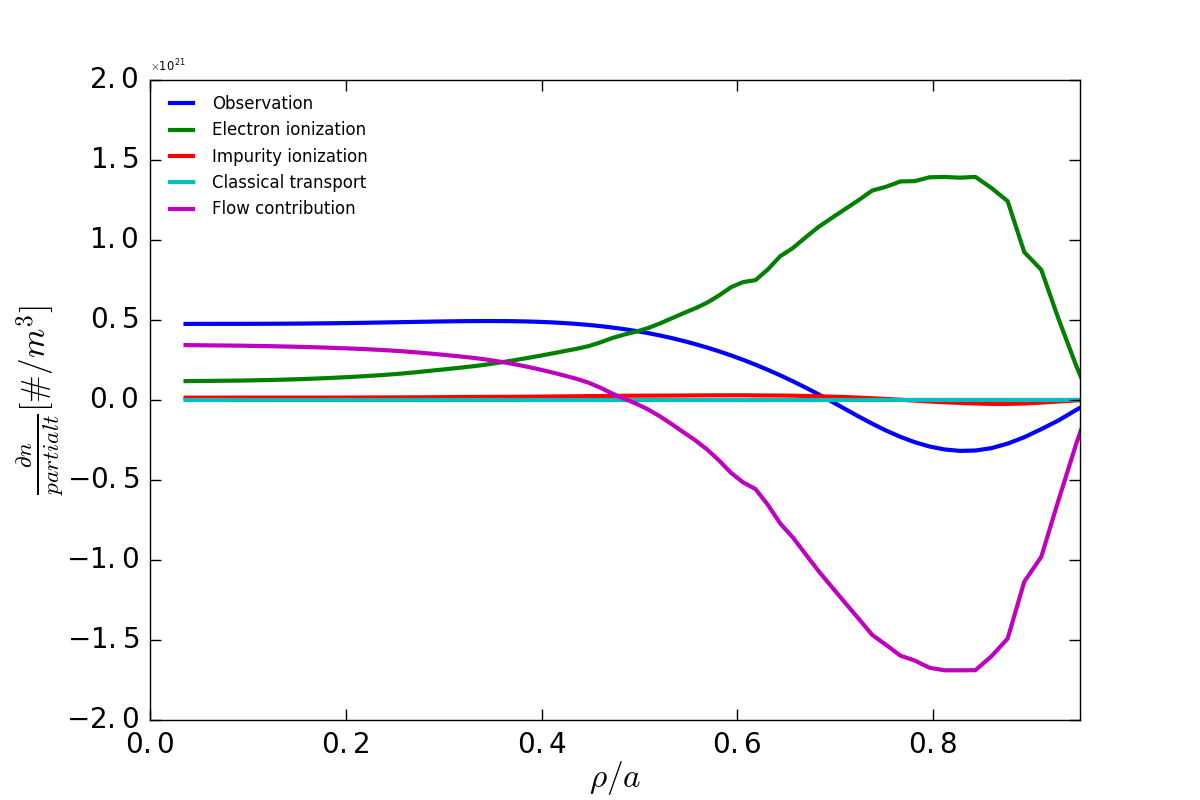
\includegraphics{ion_transport_results/density_balance.png}
    \caption{$\partialt n_e$ in MST and their sources. This particular plot presents the ensembled analysis at 14ms.}
    \label{fig:density_balance}
    %%TODO, need larger legend text.
\end{figure}

The first step is realizing that source rate mechanisms are limited. Ionization of deuterium and impurities accounts for all the available sources of electrons. However, particle flow has not been explored to the same degree. In J. Reynolds's thesis on simulating the effect of PPCD using the numerical MHD code NIMROD \cite{Reynolds2007}, he observes the simulation undergoing an inward pinch flow across the simulated plasma volume (see figure \ref{fig:NIMROD_pinch}). He also refers to previous simulation studies on PPCD-like conditions showing inward pinch\cite{StuffThatReynoldCited}. More empirical on MST, PPCD drive the plasma into deep reversal and the reversal surface moves inwards during this process. Previous measurements of electron density using FIR also show the gradient region moving inwards (figure \ref{fig:Ne_gradient_pinch}), hinting at a pinch. After all, it is in the name of the configuration.

\begin{figure}
    \centering
    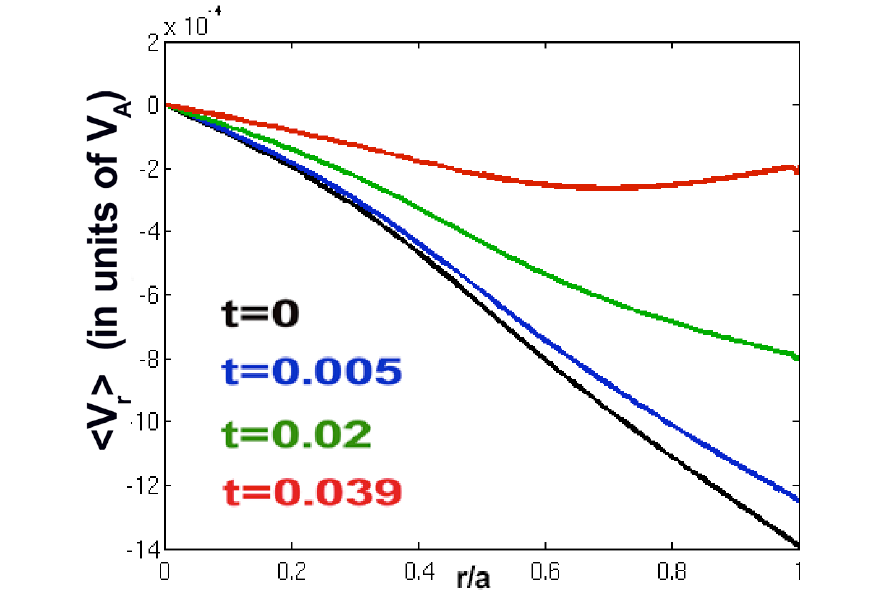
\includegraphics{ion_transport_results/reynold_pinch.png}
    \caption{Pinch velocity from J. Reynolds' simulations. Note that the simulation volume ends at the reversal surface and the Lunquist number of the simulation is lower than actual plasma conditions. (Reproduced from J. Reynolds\cite{ReynoldsThesis}). }
    \label{fig:NIMROD_pinch}
\end{figure}


Working with the hypothesis that the unaccounted for core density rise is due to a pinch flow, I use the continuity equation (equation \ref{eqn:continuity}) to calculate the particle flux needed to balance out the observations. This forms a basis for comparison with the hypothesized mechanism, \ecb drift.

\subsection{Estimating radial \ecb drift}

MST have limited ability to diagnose $\vec{E}$ field in high current plasmas. Thus the $\vec{E}$ needs to be estimated from indirectly from the $\partialt\vec{B}$ according to the Maxwell equations. The $\vec{B}$ field are calculated by the equilibrium reconstruction code MSTfit using inputs from the gap voltage measurements, edge pick up coils, and FIR polarimeter measurements. Sequential MSTfit equilibrium reconstruction are used to estimated $\partialt\vec{B}$. From there $E_{pol}$ can be calculated through:
\begin{align}
   E_{pol}(\rho_v) & = -\frac{1}{\rho_v}\int_{0}^{\rho_v}\rho_v' \frac{dB_{tor}}{dt} d\rho_v'
\end{align}
where it is taken as a boundary condition that the $E_{pol}$ is zero at the magnetic axis.

The calculation of $E_{tor}$ is slightly more complicated, as it is a function of major radius and not $\rho_v$. The voltage measurement ($V_{PG}$) across the poloidal gap on MST (a cut in the vacuum vessel along its intersection with the poloidal plane) is a reflection of the toriodal E field at the wall and serves as the boundary condition for the integration. $E_{tor}(R, Z=0)$ along the Z = 0 plane is determined as a function of major radius (R) through:
\begin{align}
\oint_S \vec{E}\cdot d\vec{l} &= -\iint \frac{\partial}{\partial t}\vec{B}\cdot d\vec{s}\\
E_{tor}(R) 2\pi R &= -\int_0^{2\pi}\int_{R_{in}}^{R}R'\frac{\partial B_{pol}}{\partial t} d\phi'dR' - V_{PG}\\
E_{tor}(R) &= -\frac{1}{R}\int_{R_{in}}^{R}R'\frac{\partial B_{pol}}{\partial t} dR' - \frac{V_{PG}}{2\pi R}\label{eqn:E_tor}
\end{align}
where $R$ refers to the major radius, and $R_{in}$ is the major radius at the inboard wall. To incorporate into the 1-D approximation, the inboard and outboard $E_{tor}$ is averaged according to their flux surface subsequently. From these, we can calculate the radial \ecb flux,
\begin{align}
    \Gamma_{\vec{E} \times \vec{B}} &= n_e v_{\mecb} \nonumber \\
    &= n_{e} \frac{E_{pol}B_{tor} - E_{tor}B_{pol}}{B^2}
\end{align}
The result of this calculation is shown in figure \ref{fig:eb_v}. This can be compared with the observed flux calculated from the continuity equation (figure \ref{fig:eb_v}). The result show that \ecb is a good explanation for the inwards flow needed to balance out the observations. Hence, the $\partialt n_e$ rise in the core can now be accounted for in such a way that the associated ion temperature is no longer arbitrary, since \ecb flow is ambipolar.

\begin{figure}
    \centering
    \includegraphics{ion_transport_results/eb_v.png}
    \caption[Calculated \ecb pinch velocity]{Calculated \ecb pinch velocity. The velocity is plotted to the reversal surface. Compares well with MHD simulations results in figure \ref{fig:NIMROD_pinch} qualitatively. }
    \label{fig:eb_v}
\end{figure}
\begin{figure}
    \centering
    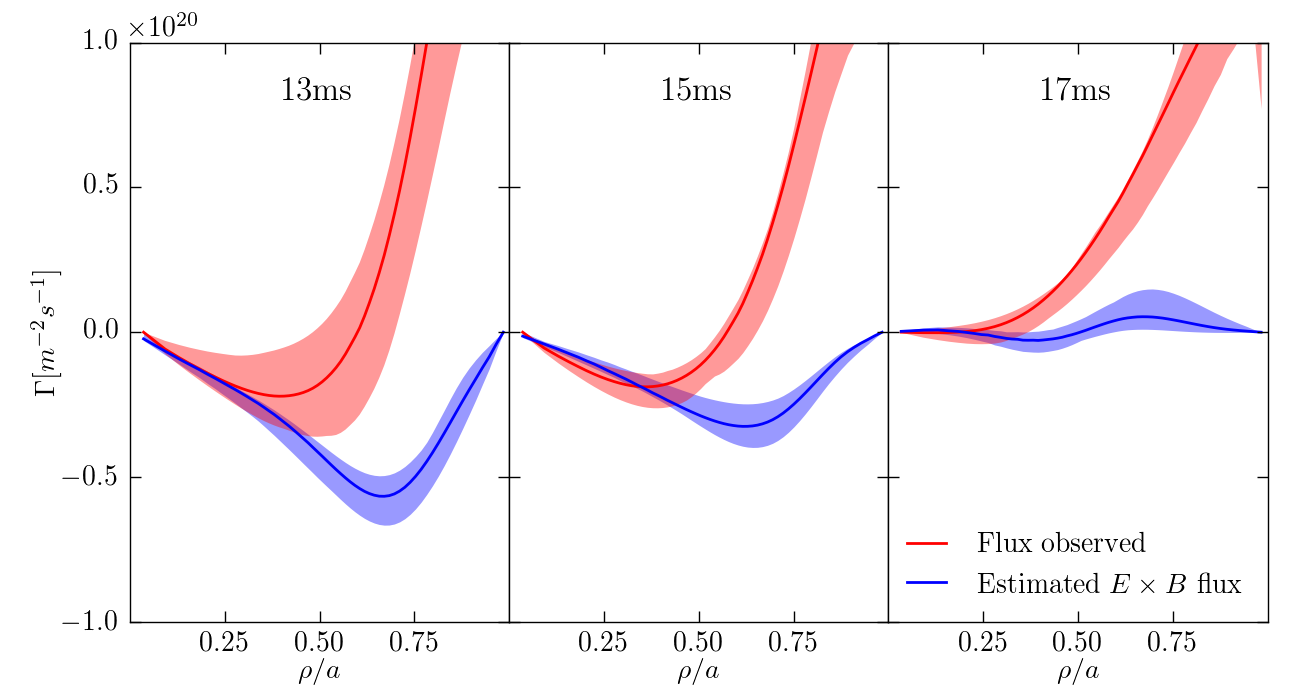
\includegraphics{ion_transport_results/flux_comp.png}
    \caption[\ecb flux compared to measured flux]{\ecb flux compared to the observed flux. 'Observed' flux is that implied by the continuity equation though $\partialt n$ and source rate observations. The two match until the mid-radius. The outer areas of the plasma is dominated by an outward anomalous particle flux. The outward flux at the edge is consistent with previous estimates\cite{TakashisSource}. }
    \label{fig:eb_v}
\end{figure}

\subsection{Flow effects on thermal transport}

The effects of the flow can be calculated via the method laid out in section \ref{sec:flow_effects}. It is useful reiterate the two components of the flow effect. One has to do with the conservation of the energy being carried by the ions. This term brings energy into the core, but generally will result in cooling, whereas it brings energy out of the edge (loss to wall), but is general increasing temperature as they are 'replaced' by ions flowing out from mid-radius. The other term is the compressional work by the \ecb drift in varying fields. This is calculated from the estimated drift velocity, and is a mostly positive term, and since it doesn't not have density effects, it represents a temperature increase. The details of these two terms are presented in figure \ref{fig:flow_power_terms}. 

\begin{figure}
    \centering
    \includegraphics{ion_transport_results/flow_power_terms.png}
    \caption[Power terms resulting from radial ion flow]{Power terms resulting from radial ion flow.}
    \label{fig:flow_power_terms}
\end{figure}